%%%%%%%%%%%%%%%%%%%%%%%%%%%%%%%%%%%%%%%%%%%%%%%%%%%%%%%%%%%%%%%%%%%%%%%%%%%%%%%%
%%%%%%%%%%%%%%%%%%   Vorlage für eine Abschlussarbeit   %%%%%%%%%%%%%%%%%%%%%%%%
%%%%%%%%%%%%%%%%%%%%%%%%%%%%%%%%%%%%%%%%%%%%%%%%%%%%%%%%%%%%%%%%%%%%%%%%%%%%%%%%

% Erstellt von Maximilian Nöthe, <maximilian.noethe@tu-dortmund.de>
% ausgelegt für lualatex und Biblatex mit biber

% Kompilieren mit
% latexmk --lualatex --output-directory=build thesis.tex
% oder einfach mit:
% make

\documentclass[
  12pt,          % Schriftgröße
  tucolor,       % remove for less green,
  %BCOR=12mm,     % 12mm binding corrections, adjust to fit your binding
  %parskip=half,  % new paragraphs start with half line vertical space
  open=any,      % chapters start on both odd and even pages
  cleardoublepage=plain,  % no header/footer on blank pages
]{tudothesis}

\usepackage[a4paper,       % Papierformat
top=3.5cm,     % Top margin
bottom=3.5cm,  % Bottom margin
left=2.5cm,    % Left margin
right=2.5cm,   % Right margin
]{geometry}


% Warning, if another latex run is needed
\usepackage[aux]{rerunfilecheck}

% just list chapters and sections in the toc, not subsections or smaller
\setcounter{tocdepth}{1}

%------------------------------------------------------------------------------
%------------------------------ Fonts, Unicode, Language ----------------------
%------------------------------------------------------------------------------
\usepackage{fontspec}
\defaultfontfeatures{Ligatures=TeX}  % -- becomes en-dash etc.
\setlength\parindent{0pt}

% load english (for abstract) and ngerman language
% the main language has to come last
\usepackage[ngerman,american]{babel}

% intelligent quotation marks, language and nesting sensitive
\usepackage[autostyle]{csquotes}

% microtypographical features, makes the text look nicer on the small scale
\usepackage{microtype}

%------------------------------------------------------------------------------
%------------------------ Math Packages and settings --------------------------
%------------------------------------------------------------------------------

\usepackage{amsmath}
\usepackage{amssymb}
\usepackage{mathtools}

% Enable Unicode-Math and follow the ISO-Standards for typesetting math
\usepackage[
  math-style=ISO,
  bold-style=ISO,
  sans-style=italic,
  nabla=upright,
  partial=upright,
  warnings-off={mathtools-colon,mathtools-overbracket}, % suppress some unnecessary warnings
]{unicode-math}
\setmathfont{Latin Modern Math}

% nice, small fracs for the text with \sfrac{}{}
\usepackage{xfrac}


%------------------------------------------------------------------------------
%---------------------------- Numbers and Units -------------------------------
%------------------------------------------------------------------------------

\usepackage[
  locale=US,
  separate-uncertainty=true,
  per-mode=symbol-or-fraction,
]{siunitx}

%------------------------------------------------------------------------------
%-------------------------------- tables  -------------------------------------
%------------------------------------------------------------------------------

\usepackage{booktabs}       % \toprule, \midrule, \bottomrule, etc

%------------------------------------------------------------------------------
%-------------------------------- graphics -------------------------------------
%------------------------------------------------------------------------------

\usepackage{graphicx}
% currently broken
% \usepackage{grffile}

% allow figures to be placed in the running text by default:
\usepackage{scrhack}
\usepackage{float}
\floatplacement{figure}{htbp}
\floatplacement{table}{htbp}

% keep figures and tables in the section
\usepackage[section, below]{placeins}

% allows to include PDFs as full pages
\usepackage{pdfpages}

% Set the PDF Version of this document to 1.7 (1.4 is the current default)
% This is needed so that PDFs with Version >1.5 can be included
\pdfvariable minorversion=7

%------------------------------------------------------------------------------
%---------------------- customize list environments ---------------------------
%------------------------------------------------------------------------------

\usepackage{enumitem}

%------------------------------------------------------------------------------
%------------------------------ Bibliographie ---------------------------------
%------------------------------------------------------------------------------

\usepackage[
  backend=biber,   % use modern biber backend
  autolang=hyphen, % load hyphenation rules for if language of bibentry is not
                   % german, has to be loaded with \setotherlanguages
                   % in the references.bib use langid={en} for english sources
]{biblatex}
\addbibresource{references.bib}  % the bib file to use
\DefineBibliographyStrings{american}{andothers = {{et\,al\adddot}}}  % replace u.a. with et al.


% Last packages, do not change order or insert new packages after these ones
\usepackage[pdfusetitle, unicode, linkbordercolor=tugreen, citebordercolor=tugreen]{hyperref}
\usepackage{bookmark}
\usepackage[shortcuts]{extdash}

%------------------------------------------------------------------------------
%-------------------------    Angaben zur Arbeit   ----------------------------
%------------------------------------------------------------------------------

\author{Jonas Ollesch}
\title{Identifying AI generated images using CNNs across different epochs}
\date{Submission: July 29, 2024}
\chair{Machine Learning Lecture}
\division{Fakultät Physik}
%\submissiondate{July 29 2024}

% tu logo on top of the titlepage
\titlehead{
\includegraphics[height=1.5cm]{logos/tu-logo.pdf}}

\begin{document}
\frontmatter
\maketitle

% hier beginnt der Vorspann, nummeriert in römischen Zahlen
%\thispagestyle{plain}

\section*{Kurzfassung}
In dieser Arbeit betrachten wir die Kopplung zwischen Neutrinos als Majoranateilchen, also Teilchen, die mit ihren Antiteilchen übereinstimmen, und Majoronen, den Teilchen, die,
ähnlich wie das Higgs-Boson für alle anderen Teilchen, Neutrinos ihre Masse verleihen.
Über den hypothetischen neutrinolosen Doppelbetazerfall und Beobachtungen der Spektren und Luminositäten von Supernovae lassen die die zulässigen Kopplungparameterbereiche limitieren.
Es gelingt uns, mithilfe beobachteter Daten der Supernova SN1987A, die Kopplungsparameter $|g_{i j}|$ auf $|g_{i j}| < \frac{\num{0.83} \cdot 10^{-8}}{m_J} \,\si{\mega\eV}$ 
in einem Bereich von $\SI{100}{\eV} < m_J < \SI{100}{\mega\eV}$ einzuschränken.
Gemeinsam mit der Neutrinomassengrenze von $m_1 < \SI{0.8}{\eV}$ aus dem KATRIN-Experiment und der Einschränkung $g_1 < 10^{-4}$ aus einer Betrachtung der Neutrinospektren lässt sich der in \autoref{fig:exclusionregionfinal}
dargestellte Parameterbereich ausschließen. \\
Nach abschließendem Vergleich mit den von Hau Zhang in \cite{hauhau} aus dem neutrinolosen Doppelbetazerfall erhaltenen Obergrenzen auf die Kopplung $g_{ee}$ mit $\num{0.4} \, \cdot \, 10^{-5} < g_{ee} < \num{0.9} \, \cdot \, 10^{-5}$ sehen wir, dass
der Doppelbetazerfall die von uns ermittelte Ausschlussregion nicht weiter einschränkt.

\section*{Abstract}
\begin{foreignlanguage}{english}
In this thesis, we discuss the coupling between neutrinos as majorana particles, thus particles that coincide with their anti particles, and majorons, the particles that, like the Higgs boson does for all other
particles, give the neutrios their mass.
The valid coupling parameter regions can be limited by discussing the hypothetical neutrinoless double beta decay and observed supernova spectra and their luminosities.
We succeed in limiting the coupling parameters $|g_{i j}|$ to $|g_{i j}| < \frac{0.83 \cdot 10^{-8}}{m_J} \,\si{\mega\eV}$ in a range of $\SI{100}{\eV} < m_J < \SI{100}{\mega\eV}$.
Together with the neutrino mass limit of $m_1 < 0.8 \,\si{\eV}$, obtained from the KATRIN experiment, and the restriction $g_1 < 10^{-4}$ from neutrino spectra, we gain the exclusion region represented in
\autoref{fig:exclusionregionfinal}. \\
By comparing our results to the upper limits on $g_{ee}$ from neutrinoless double beta decay, obtained by Hau Zhang in \cite{hauhau} with $\num{0.4} \, \cdot \, 10^{-5} < g_{ee} < \num{0.9} \, \cdot \, 10^{-5}$, we see no further
modification of the assumed exclusion region.
\end{foreignlanguage}

\tableofcontents

\mainmatter
% Hier beginnt der Inhalt mit Seite 1 in arabischen Ziffern
\chapter{Introduction and Motivation}
\label{ch:intro}

Over the last few years, the quality of AI generated content has improved unfathomably.
Be it the appearance of generative model like \textit{Chat-GPT}, an almost human chatbot seemingly able to answer every question,
or methods such as \textit{Stable Diffusion} which can be used to generate almost convincingly real images, 
AI has by now taken a hold in almost every field. 
The average consumer thus gains access to an entirely new level of convenience. \\

Still, this poses perhaps as many dangers as it provides merits.
One of those dangers can be seen every while just writing this report - as GitHub's \textit{Copilot} is always eager to provide a "helpful" suggestion,
luring the author to just stop thinking and let the AI do the work. \\

Here, however, we will deal with a different kind of problem: how can it be ensured that AI generated images are correctly identified?
As of now, it is still possible, at least for the more-informed, to differentiate between generated and real images, but considering the rapid progress over the last years,
it is unlikely to remain that way for much longer. \\ %maybe reference the generated videos from earlier this year here







\chapter{The Dataset}
\label{ch:dataset}

The dataset used in this project is the \textit{AI-ArtBench} dataset from Kaggle \cite{aiartbench}.
It contains over $180000$ images, of which $60000$ are human drawn and the rest are AI generated.
The images are pre-split into train and test data, with around $155015$ and $30000$ used for training and testing, respectively.
Further, the dataset is divided into different subfolders, each containing images from a different epoch.
Those epochs are: Art Nouveau, Baroque, Expressionism, Impressionism, Post impressionism, Realism, Renaissance, Romanticism, Surrealism, Ukiyo-e. \\

It should be noted that the AI generated images in this dataset were generated using two different models, Latent Diffusion (LD) and Standard Diffusion (SD).
The exact machinations of those models are not relevant here, nor is it our aim to differentiate between them.
Thus, the AI generated images were thrown together into a single category.
Another minor change made to the dataset was to cap all folder at $5000$ images, at least before fusing the LD and SD folders.
This is the number of images for the folders containing the human drawn art.
While the inconsistency in the number of images per epoch was minute, we thought it sufficient to sacrifice a few images for the sake of stability.
Additionally, some images had to be resized, as, contrary to what the dataset's description claims, some images were indeed not square $256 \times 256$ images,
but rectangular instead.
Those images were cropped to $256 \times 256$ pixels. \\

\begin{figure}
    \centering
    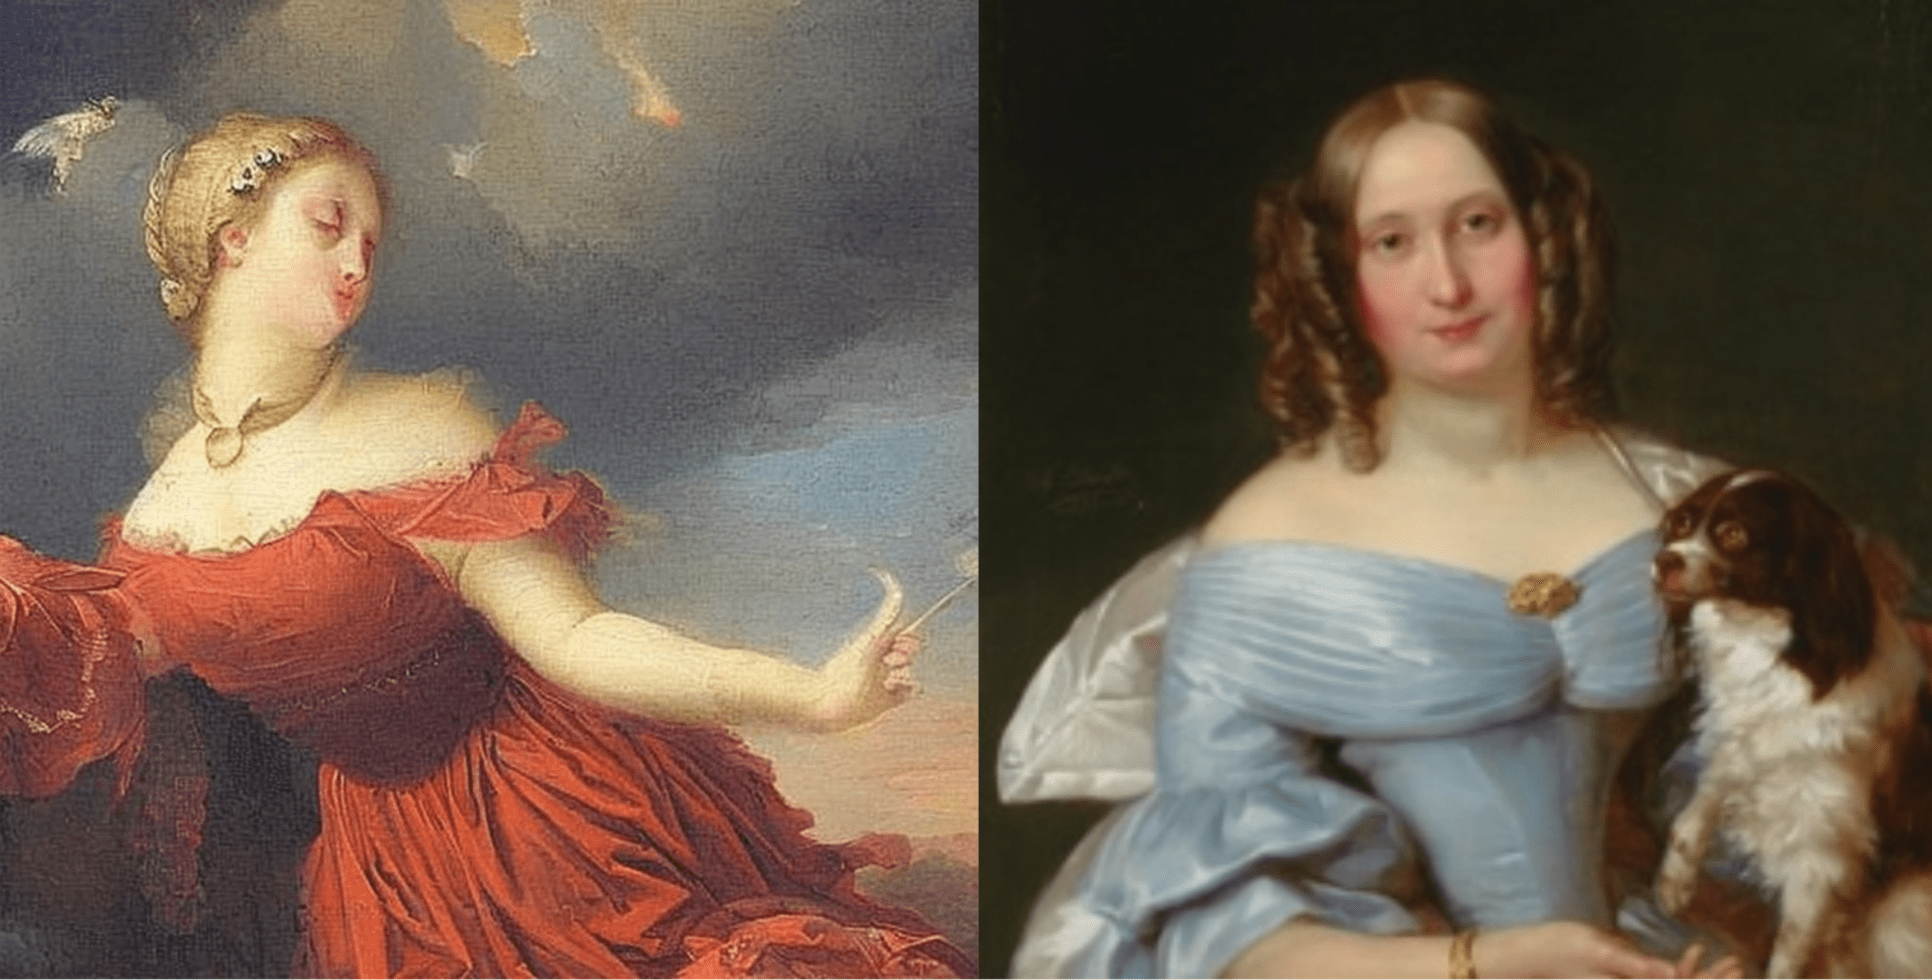
\includegraphics[width=0.5\textwidth]{images/Example_images.png}
    \caption{Example images from the dataset with the AI generated image on the left and the human-drawn on the right \cite{aiartbench}.}
    \label{fig:example_images}
\end{figure}

Concerning previous work, we found one work on this exact dataset by Kaggle user \textit{nibrastuhh} \cite{useraiartbench}, who used
a neural network to classify the images, reaching an accuracy of over $90\%$.
They, however, focused on merely the classification of the images, while we are going to be focusing more on the details.
Typically, other work in the same direction focuses on detecting AI generated photographs, not art.


\chapter{Using a CNN to solve the Problem}
\label{ch:solution}

\chapter{Results and Conclusion}

\section{Results}
\label{sec:results}


\appendix
% Hier beginnt der Anhang, nummeriert in lateinischen Buchstaben
\chapter{Anhang}

\backmatter
\printbibliography

\cleardoublepage
% From https://www.tu-dortmund.de/studierende/im-studium/pruefungsangelegenheiten/allgemeine-vordrucke/
%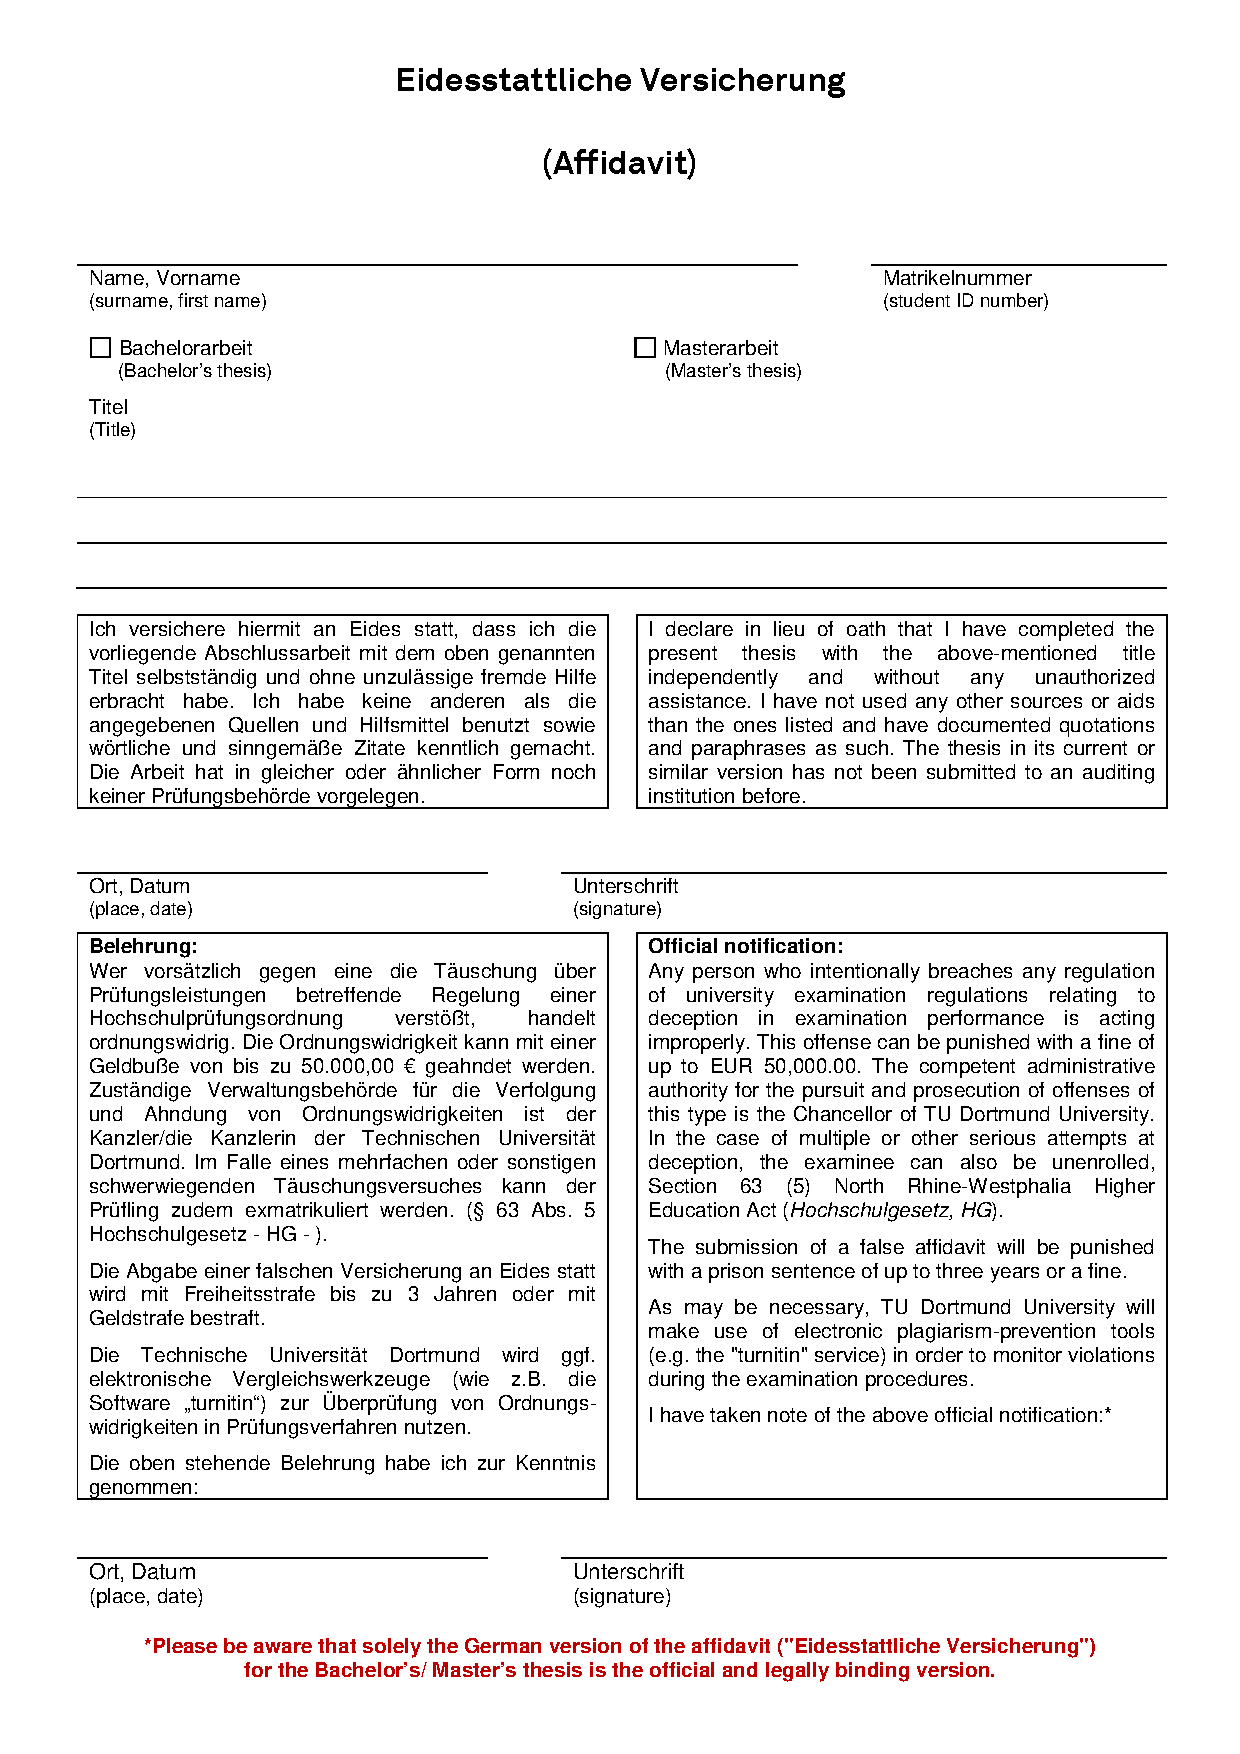
\includepdf{content/Eidesstattliche_Versicherung.pdf}

\end{document}
